\documentclass[border=5pt]{standalone}
\usepackage{fontspec}
\setmainfont{Times New Roman}
\setmonofont{Courier New}
\usepackage{amsmath,graphicx,fancyvrb}
\setlength{\fboxsep}{7pt}
\setlength{\fboxrule}{0.5pt}
\begin{document}
\begin{minipage}{510pt}
\fontsize{10}{12}\selectfont
\begin{minipage}[t]{225pt}
\vspace{0pt}\textbf{(a) Stored verification links}\par\smallskip
\begin{Verbatim}[fontsize=\fontsize{7.5}{9.6}\selectfont]
class VerificationCondition(ModelObject):
    measure = Property()
    target = Property()

condition = VerificationCondition(
    "minimum", battery.bol_energy,
    Property("self.parent.required", "J"),
    "measure >= target")
\end{Verbatim}
\end{minipage}\hfill
\begin{minipage}[t]{275pt}
\vspace{0pt}\textbf{(b) GUI verification condition}\par\smallskip
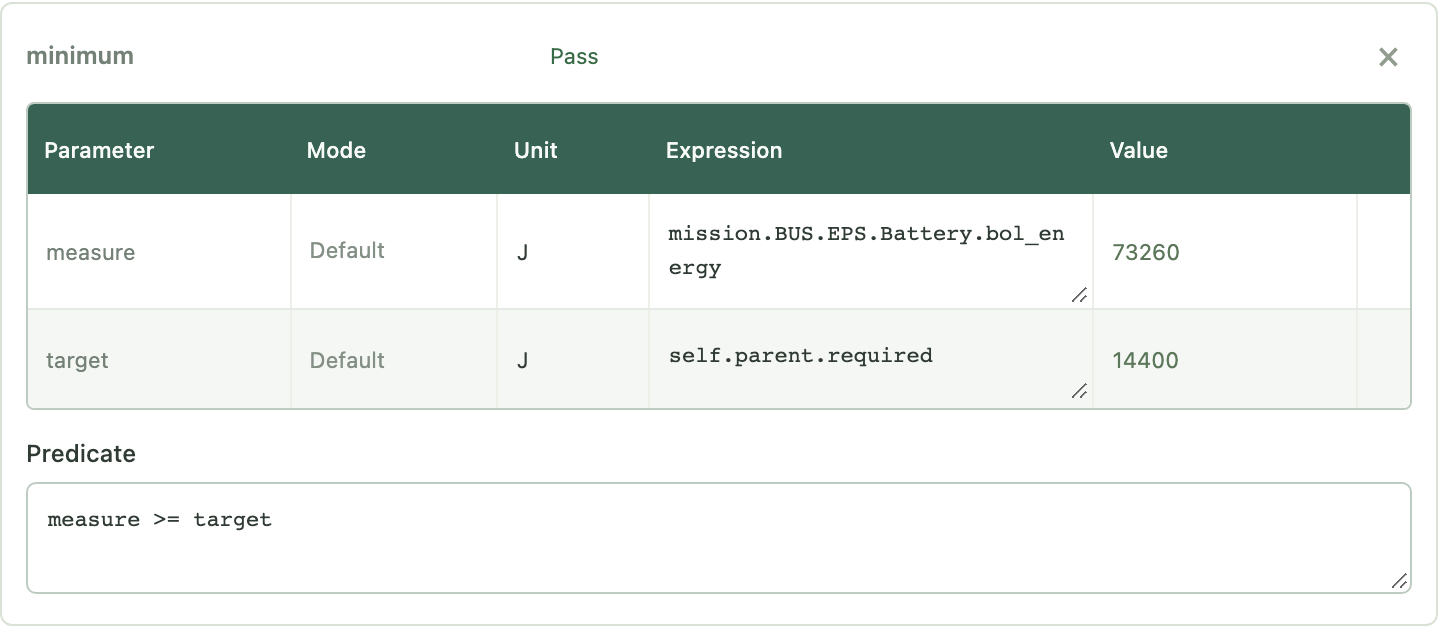
\includegraphics[width=275pt]{verification-condition.png}\end{minipage}\par\medskip\textbf{(c) Requirement evaluation method}\par
\begin{Verbatim}[fontsize=\fontsize{8}{10.24}\selectfont]
def verify(self, *, mode=None):
    return VerificationReport(self.mission, tuple(
        condition.evaluate(mode=mode)
        for condition in self.conditions))
\end{Verbatim}

\end{minipage}
\end{document}
